\subsection{Devices Configuration}

\subsubsection*{R5}
The Router5 is a clone of the Router1.
The network of this router is composed by two enabled adapters:
\begin{itemize}
	\item Adapter 1: Internal Network (Name: intnet);
	\item Adapter 2: NAT Network (Name: NatNetwork).
\end{itemize}
After the start of the machine it is setted with this commands:

\lstinputlisting[language=bash]{cfg_files/r5.txt}

\subsubsection*{R1}
\lstinputlisting[language=bash]{cfg_files/r1.txt}

\subsubsection*{R2}
\lstinputlisting[language=bash]{cfg_files/r2.txt}

\subsubsection*{R3}
\lstinputlisting[language=bash]{cfg_files/r3.txt}

\subsubsection*{R4}
\lstinputlisting[language=bash]{cfg_files/r4.txt}

\subsubsection*{Kali-PC1}
\lstinputlisting[language=bash]{cfg_files/Kali-PC1_interfaces.txt}
\lstinputlisting[language=bash]{sh/PC1.sh}

\subsubsection*{Kali-PC2}
\lstinputlisting[language=bash]{cfg_files/Kali-PC2_interfaces.txt}
\lstinputlisting[language=bash]{sh/PC2.sh}

\subsubsection*{XP1}
\begin{center}
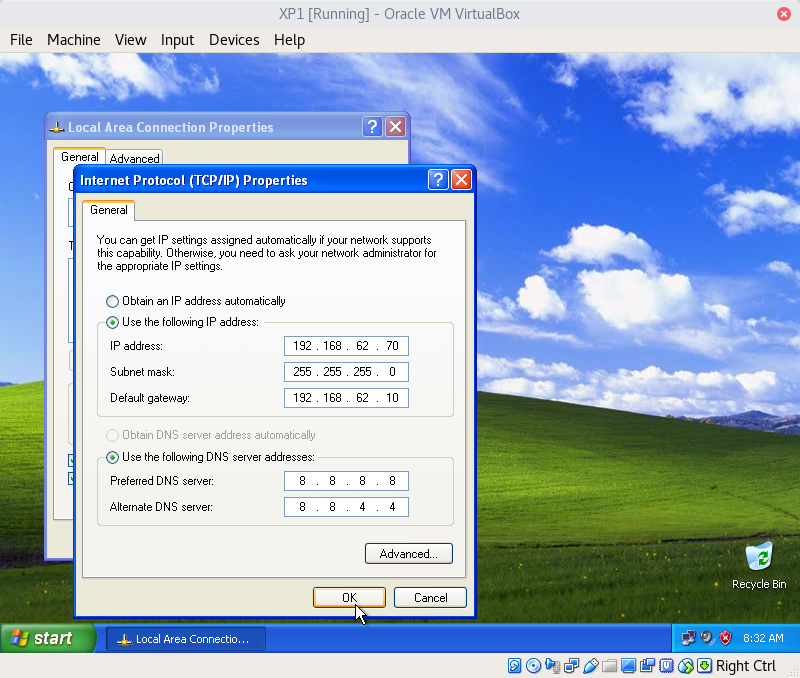
\includegraphics[width=8cm]{img/WinXPNetworkConfiguration.png}
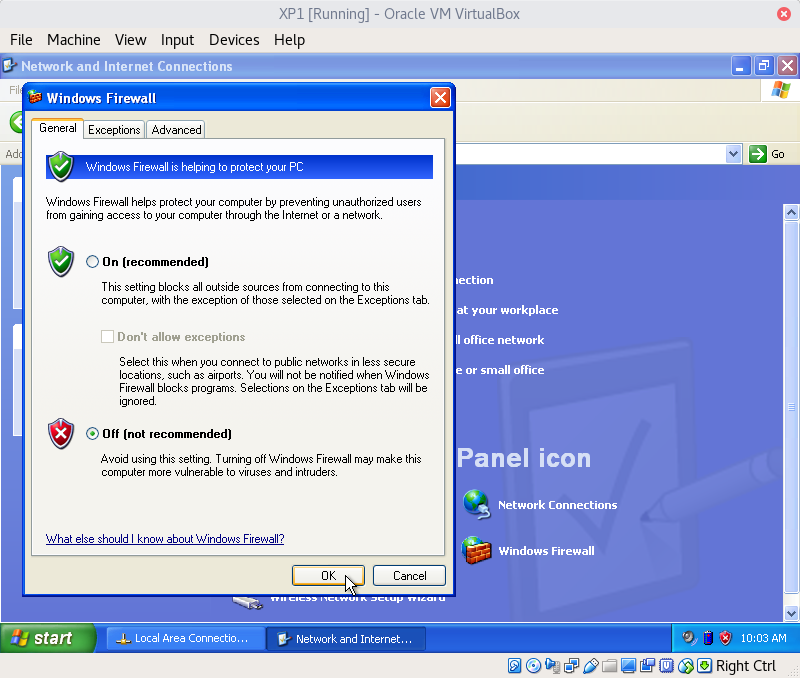
\includegraphics[width=8cm]{img/WinXPFirewallDisabled.png}\par
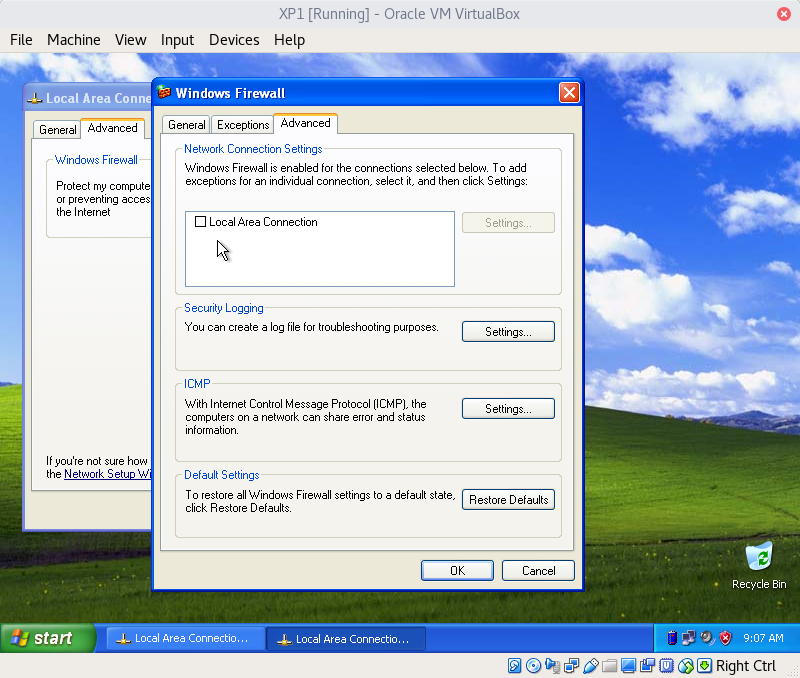
\includegraphics[width=8cm]{img/WinXPFirewallDisabledForLAN.png}
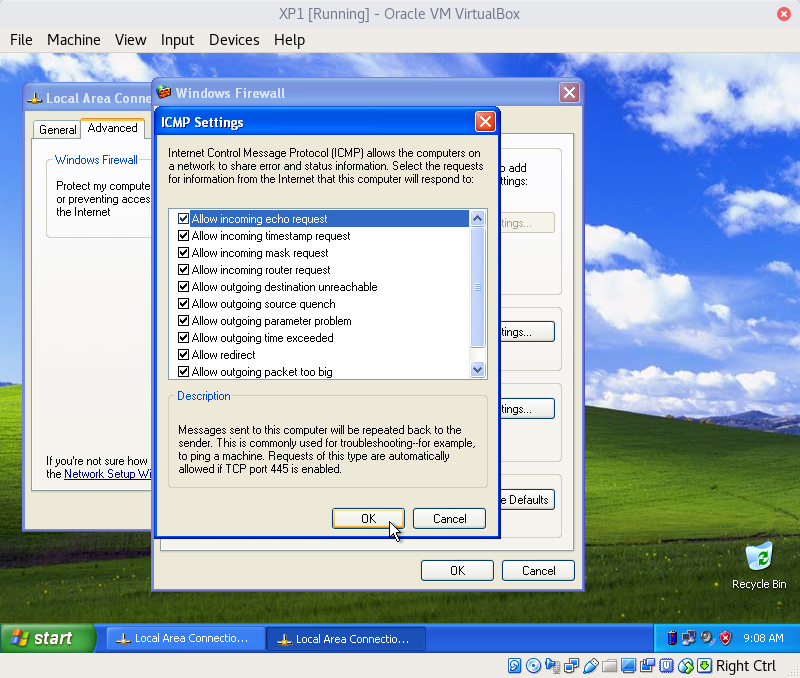
\includegraphics[width=8cm]{img/WinXPICMPAllowed.png}
\end{center}

\subsection{Testing the configuration}
Bash version of a test.\par
\lstinputlisting{sh/TestConfiguration.sh}
Now it's presented a scapy program used to test if the network was working properly before the attacks.\par
\lstinputlisting{scapy/TestConfiguration.py}
